
% --- Fig. 2 (Entropy–Curvature Atlas) ---
\begin{figure}[t]
  \centering
  \includegraphics[width=\linewidth]{figs_final/fig2_entropy_curvature.pdf}
  \caption{\textbf{Fig. 2 | Entropy–curvature atlas of symbolic regimes.} ...}
  \label{fig:fig2_entropy_curvature}
\end{figure}

% --- Fig. 4 (Translational map) ---
\begin{figure}[t]
  \centering
  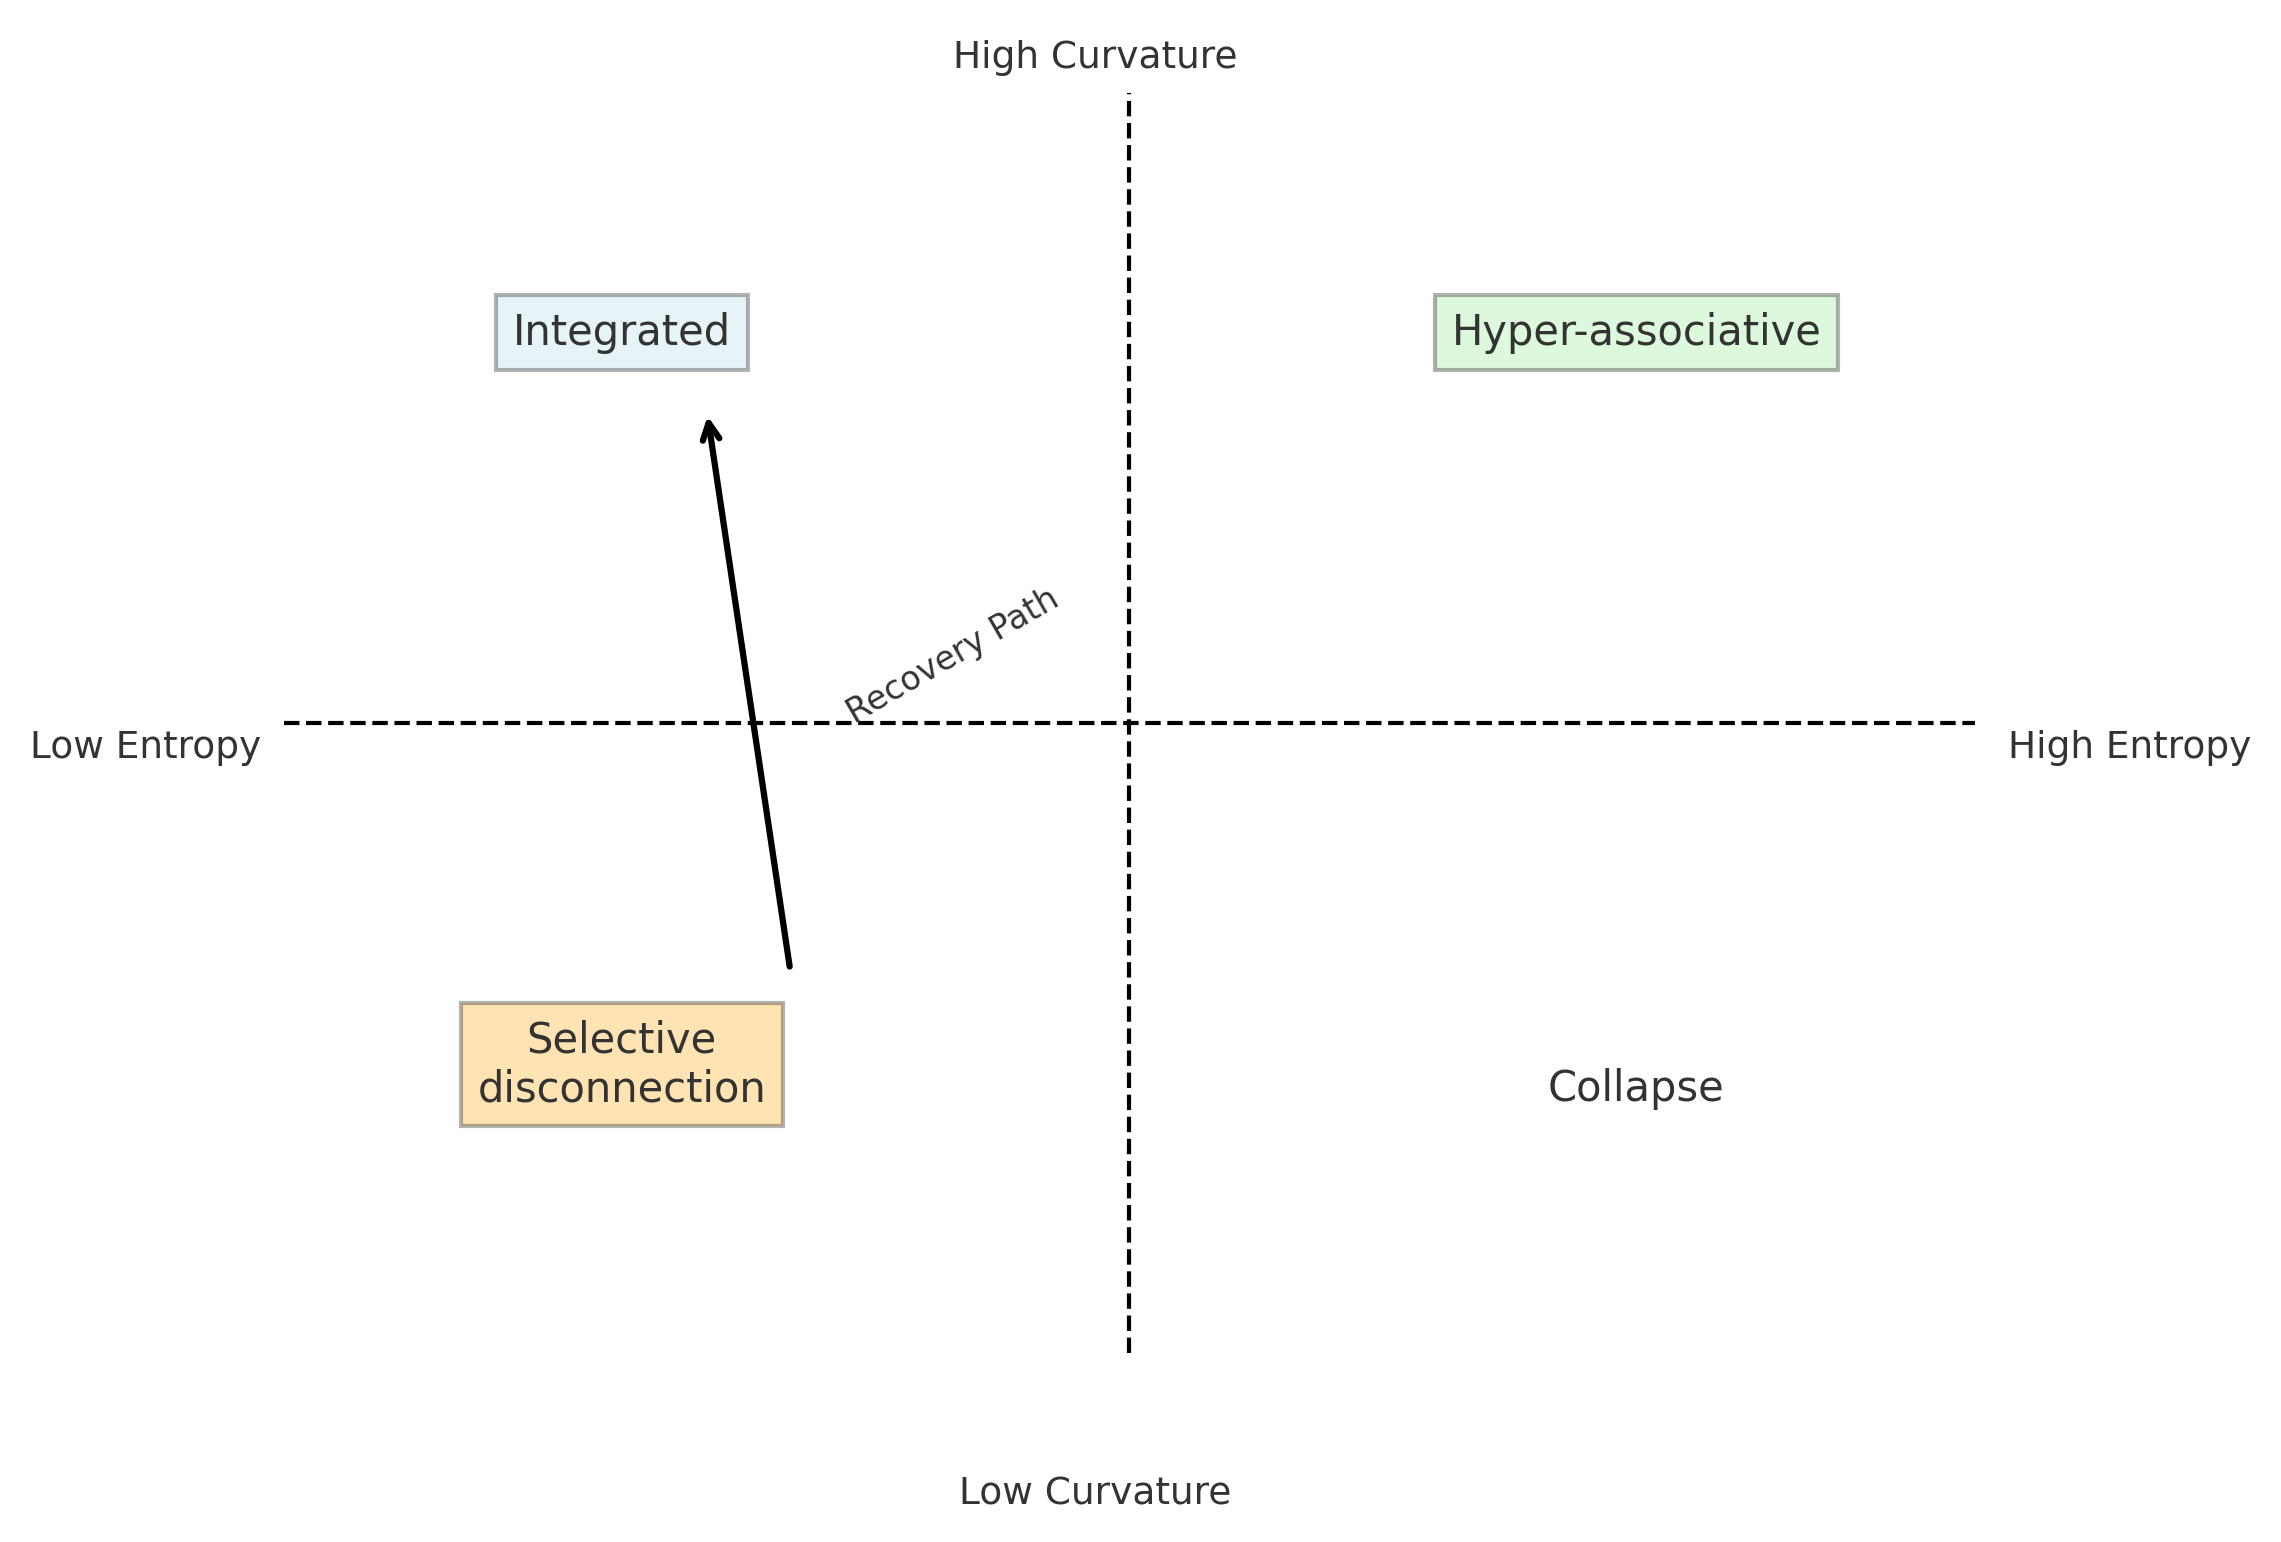
\includegraphics[width=\linewidth]{figs_final/fig4_translational.pdf}
  \caption{\textbf{Fig. 4 | Translational mapping across regimes.} ...}
  \label{fig:fig4_translational}
\end{figure}

% --- Extended Data S1 (Regime profiles) ---
\begin{figure}[t]
  \centering
  \includegraphics[width=\linewidth]{figs_final/ext_S1_regime_profiles.pdf}
  \caption{\textbf{Extended Data Fig. S1 | Regime profiles.} ...}
  \label{fig:ext_s1_profiles}
\end{figure}

% --- Extended Data S2 (Stability / Bifurcation) ---
\begin{figure}[t]
  \centering
  \includegraphics[width=\linewidth]{figs_final/ext_S2_stability.pdf}
  \caption{\textbf{Extended Data Fig. S2 | Stability and bifurcation analysis.} ...}
  \label{fig:ext_s2_stability}
\end{figure}

% --- Extended Data S3 (Degree distribution) ---
\begin{figure}[t]
  \centering
  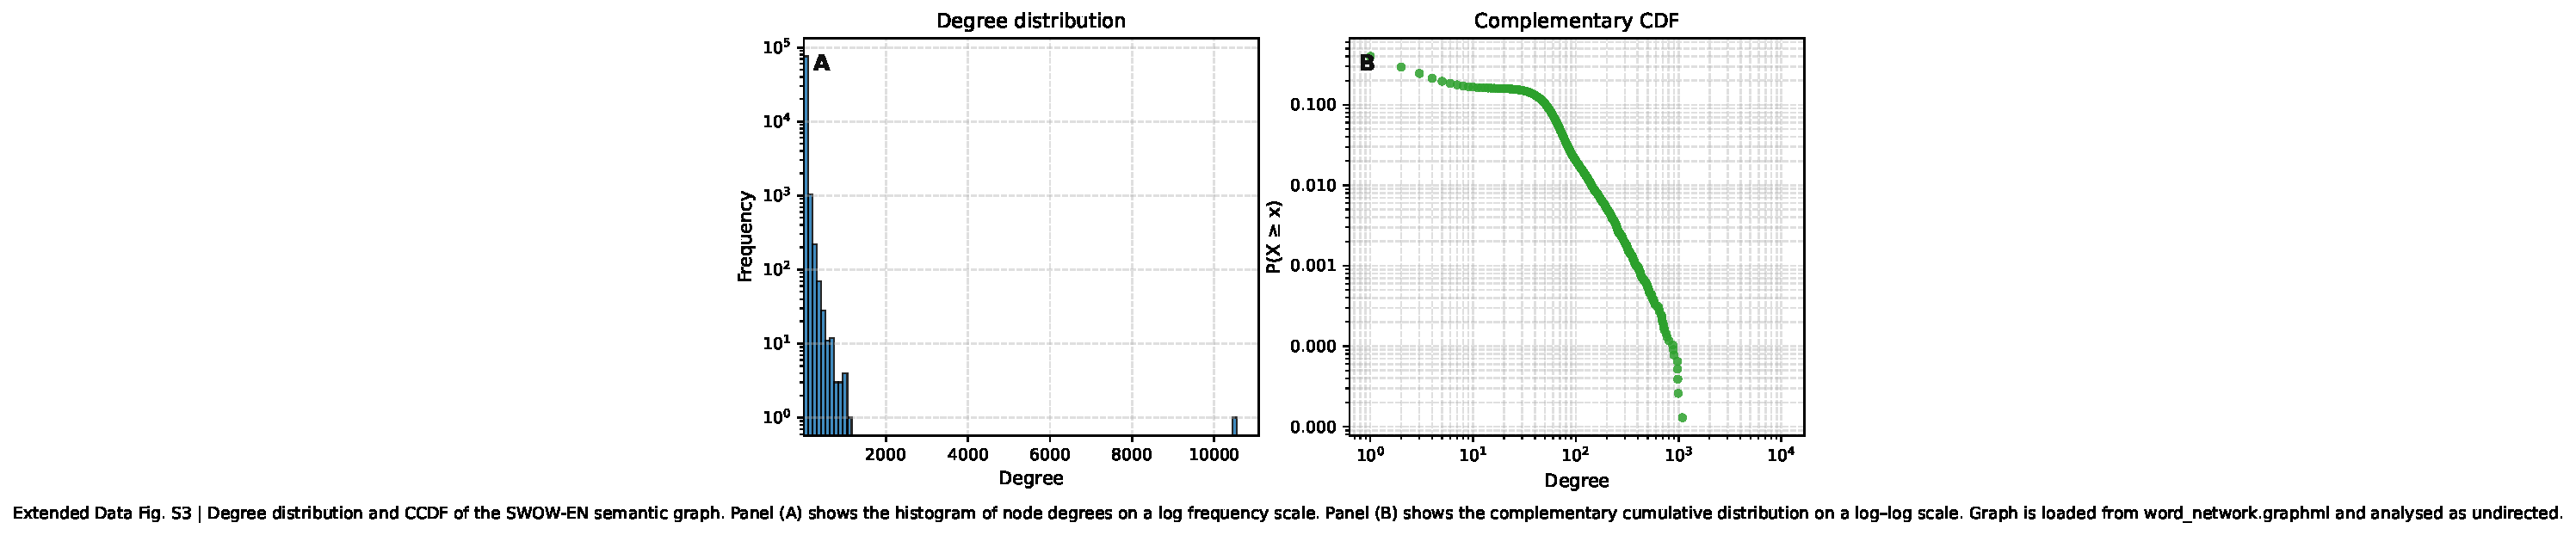
\includegraphics[width=\linewidth]{figs_final/ext_S3_degree_distribution.pdf}
  \caption{\textbf{Extended Data Fig. S3 | Degree distribution and CCDF of SWOW-EN.} ...}
  \label{fig:ext_s3_degree}
\end{figure}
